\documentclass{article}

\usepackage{graphicx}
\usepackage{tikz}
\usepackage{tikzsymbols}
\usetikzlibrary{calc,patterns,shapes.geometric}
\pagestyle{empty}
\usepackage[margin=0pt]{geometry}
\geometry{papersize={14in,12in}}

\def\centerarc[#1](#2)(#3:#4:#5){\draw[#1] ($(#2)+({#5*cos(#3)},{#5*sin(#3)})$) arc (#3:#4:#5);}

\begin{document}
	\begin{figure}
		\centering
		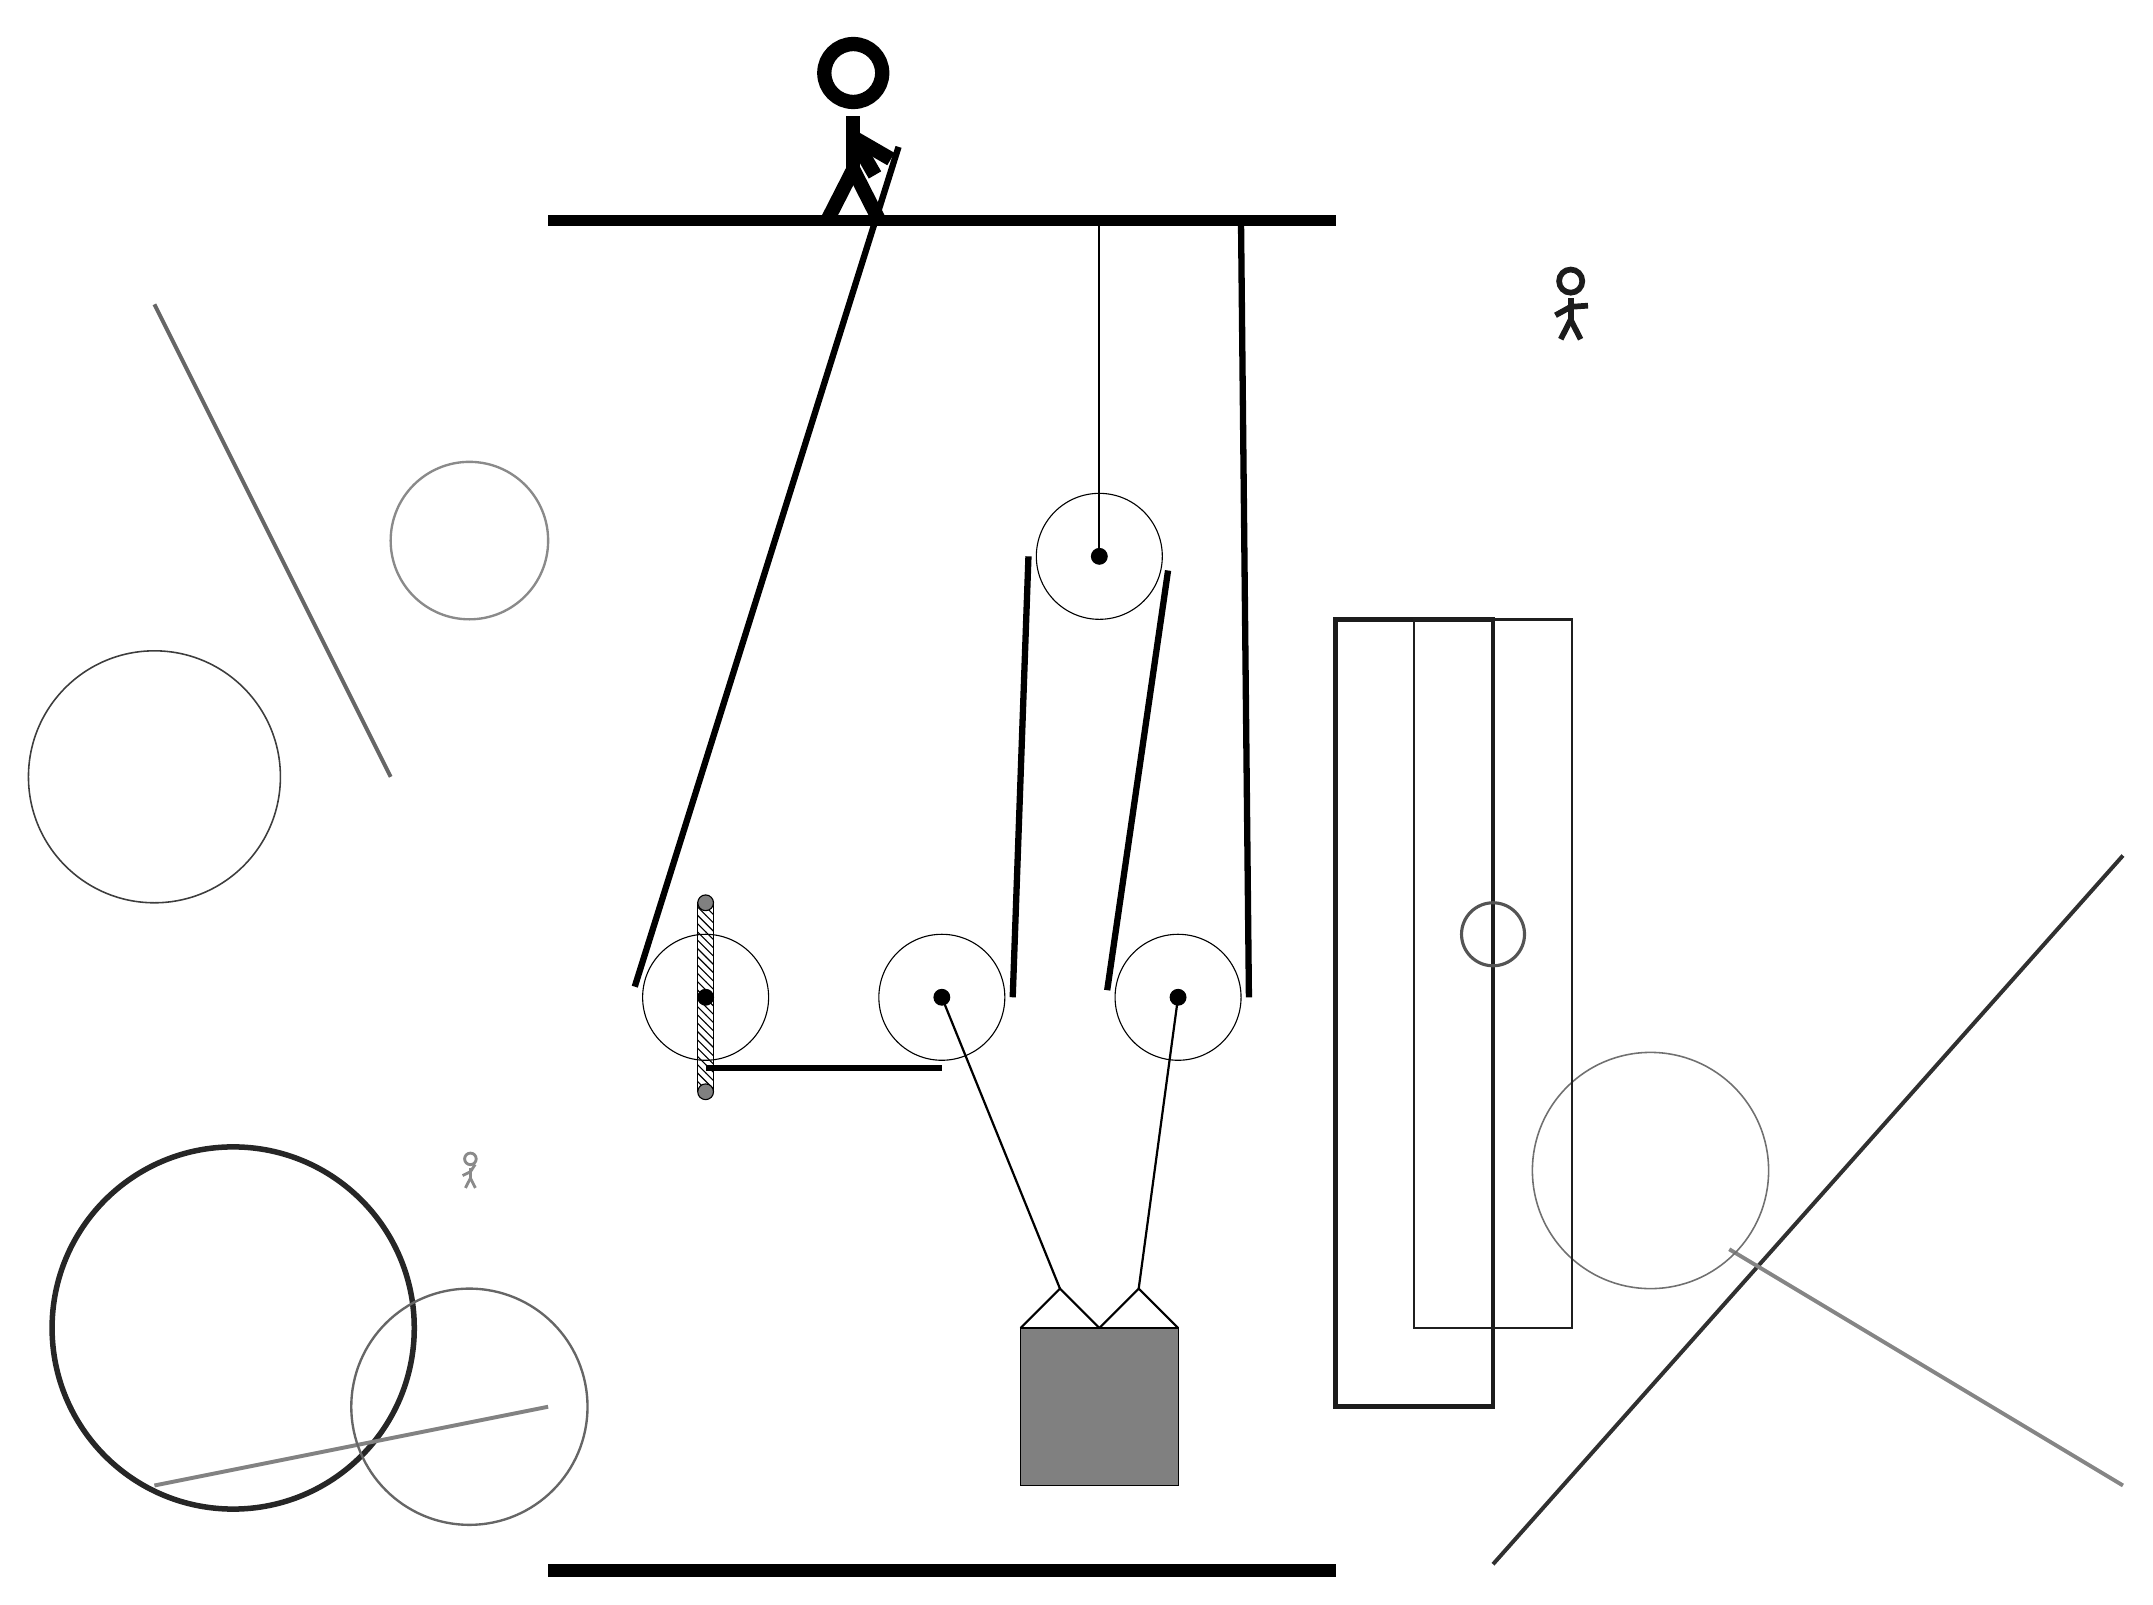
\begin{tikzpicture}
			%%%%% START %%%%%
			
			\draw[fill=black] (-4, 14) rectangle (6, 14.125);
			
			\draw (1, 4.2) circle (0.8);
			\draw[fill=black] (1, 4.2) circle (0.1);
			
			\draw (3, 9.8) circle (0.8);
			\draw[fill=black] (3, 9.8) circle (0.1);
			\draw[thick] (3, 9.8) -- (3, 14);
			
			\draw (4, 4.2) circle (0.8);
			\draw[fill=black] (4, 4.2) circle (0.1);
			
			\draw[thick] (4, 4.2) -- (3.5, 0.5);
			\draw[thick] (1, 4.2) -- (2.5, 0.5);
			\draw[thick]  (2, 0) -- (2.5, 0.5) -- (3, 0);
			\draw[thick]  (3, 0) -- (3.5, 0.5) -- (4, 0);
			\draw[fill=black!50] (2, 0) rectangle (4, -2);
			
			\draw (-2, 4.2) circle (0.8);
			\draw[fill=black] (-2, 4.2) circle (0.1);
			\draw[pattern=north west lines, pattern color=black] (-2.1, 5.4) rectangle (-1.9, 3.0);
			\draw[fill=black!50] (-2, 5.4) circle (0.1);
			\draw[fill=black!50] (-2, 3.0) circle (0.1);
			
			\draw[line width=0.8mm] (0.45, 15) -- (-2.9, 4.335);
			\centerarc[line width=0.8mm](-2, 4.2)(160:270:0.9);
			\draw[line width=0.8mm](-2, 3.3) -- (1, 3.3);
			\centerarc[line width=0.8mm](1, 4.2)(270:360:0.9);
			\draw[line width=0.8mm] (1.9, 4.2) -- (2.1, 9.8);
			\centerarc[line width=0.8mm](3, 9.8)(-20:180:0.9);
			\draw[line width=0.8mm](3.873, 9.62) -- (3.1, 4.29);
			\centerarc[line width=0.8mm](4, 4.2)(160:360:0.9);
			\draw[line width=0.8mm](4.9, 4.2) -- (4.8, 14);
			
			\node[line width=0.3mm, color=black!46] at (-5, 2) {\Strichmaxerl[2][26][57]};
			
			\draw[line width=0.5mm, color=black!60](-6, 7) -- (-9, 13);
			\draw [line width=0.7mm, color=black!85](-8, 0) circle (2.3);
			\draw[line width=0.5mm, color=black!49](-4, -1) -- (-9, -2);
			
			\draw[line width=0.5mm, color=black!81](8, -3) -- (16, 6);
			\node[line width=0.6mm, color=black!89] at (9, 13) {\Strichmaxerl[4][29][4]};
			\draw[line width=0.5mm, color=black!48](11, 1) -- (16, -2);
			\draw[line width=0.6mm, color=black!89] (8, 9) rectangle (6, -1);
			\draw [line width=0.2mm, color=black!76](-9, 7) circle (1.6);
			
			\draw [line width=0.3mm, color=black!46](-5, 10) circle (1.0);
			\draw [line width=0.2mm, color=black!56](10, 2) circle (1.5);
			\draw [line width=0.4mm, color=black!67](8, 5) circle (0.4);
			\draw[line width=0.3mm, color=black!88] (7, 9) rectangle (9, 0);
			
			\draw [line width=0.3mm, color=black!60](-5, -1) circle (1.5);
			
			\node at (-0.07, 15.2) {\Strichmaxerl[10][120][-30]};
			
			\draw[fill=black] (-4, -3) rectangle (6, -3.15);
			
			%%%%% END %%%%%
		\end{tikzpicture}
	\end{figure}	
\end{document}